\section{Current ICME Tools are Well Equipped to Integrate with an ML Framework}
The following section details how machine learning approaches can tie-in to current efforts in AM. Since the study of AM is often focused around specific problems, this section is tailored to many common areas of study within AM. Different methods of analysis and characterization for different aspects of AM all tie-in well with different machine learning algorithms. Even more so, ML can be used to automate the generation of knowledge about AM process-structure and process-property relationships. 

This article is not an exhaustive review of machine learning algorithms. The algorithms discussed were chosen because they were previously demonstrated in a materials science and engineering applications \textbf{or} because the possible application of an algorithm to AM was clear and immediate. Similarly, the additive manufacturing problems addressed are not all-encompassing. The AM problems discussed are those which the authors felt most immediately addressable with machine learning. 

%~%~%~%~%~%~%~%~%~%~%~%~%~%~%~%~%~%~%~%~%~%~%~%~%~%~%~%~%~%~%~%~%~%~%~%~%~%~%~%~%~
\subsection{Pre-Build Design}
\subsubsection{Alloy Design}
%\begin{figure}
%	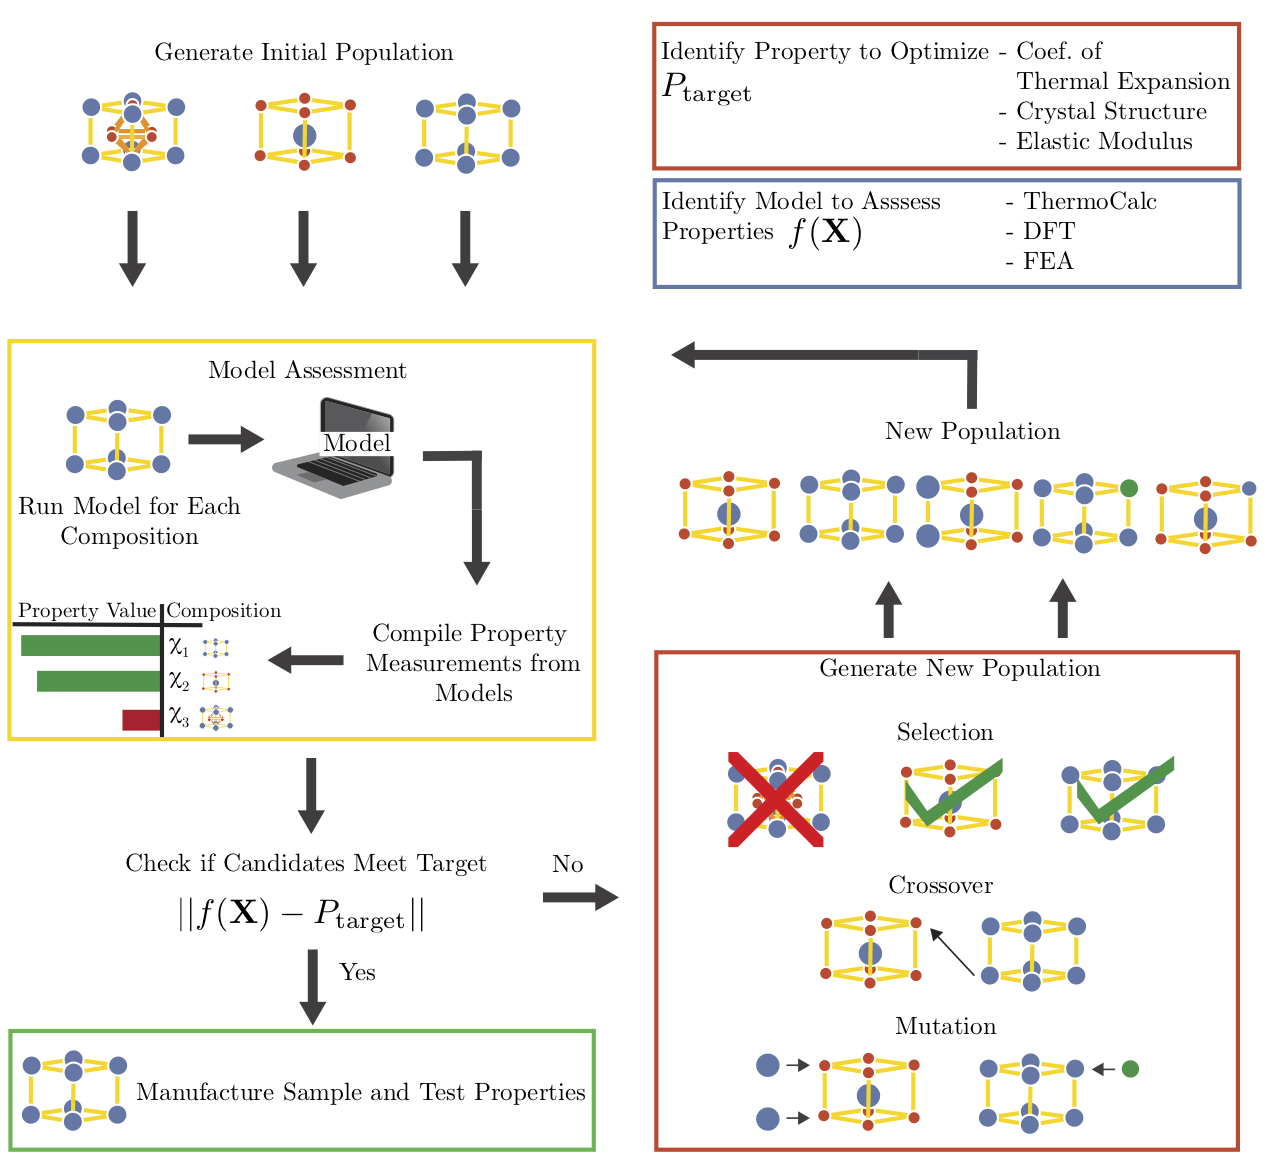
\includegraphics[width=1\linewidth]{Images/AlloyDesign}
%	\caption{}
%	\label{}
%\end{figure}
Choice of alloy impacts the physics of AM from start to finish, starting with the optics of energy sources incident on feedstock and ending with the material properties of the final part. For example, the reflected/absorbed intensity of lasers on powder beds is determined by the powder's composition \cite{Boley2016, Trapp2017}. The density of feedstock, both intra- and inter-granular density, plays a role in final part density \cite{Bi2013}. Conduction modes in the melt are partially determined by the thermal properties of the alloy \cite{Martin2017}. All of this is not to mention that different alloys exhibit different solidification kinetics, which can lead to drastically different microstructures after manufacture \cite{Collins2016}. 

Problems in the additive process can also be linked to composition such as vaporization of constituent elements due to rapid thermal fluxes, impacting the stoichiometry of melt pools and, ultimately, quality \cite{Brice2018}. Traditional engineering alloys sometimes need to be altered to improve compatibility with AM. Searching for new alloys specifically for AM may also be fruitful, as unique strengthening mechanisms can arise \cite{Brice2018, Wang2017}. Designing alloys for AM -- either altering currently used alloys or starting from scratch -- requires taking into consideration the compatibility of alloys' physical properties with AM. Alloy design for AM must take into consideration general alloy properties, like melting point, to feedstock-level properties, like vaporization temperature, to bulk alloy properties, like strength. Much of this information has been collated into databases that are compatible with design for AM. Alloy designers from AM should take advantage of these databases to search for new alloys for use in additive. 

Databases exist that contain alloy properties ranging from the reflectivity of the alloy to the mechanical properties of alloys in bulk. The International Crystal Structure Database (ICSD) contains crystallographic information for millions of compositions. The Linus Pauling files contains a range of material information, from atomic properties like radius and electron valency to crystallographic level information \cite{Villars1998}. In modern day, large databases such as AFLOWLib \cite{Curtarolo2012a}, the Materials Project \cite{Jain2013} and more allow users to search through large databases of relevant alloy information to find one that matches a desired property. Searching through large databases of information to find optimal compositions for manufacturing is actually one of the earliest materials informatics problems ever addressed. Methods exist to perform these searches in a fast, automated way. These methods are referred to as database mining, a data-driven materials design approach.

A study by Martin et al. used database mining to find micronucleants for Al alloys in powder bed manufacturing \cite{Martin2017}. Part of the design process is identifying which alloy properties are important for the desired application. Heterogeneous nucleation of Al grains was the desired outcome of Martin's study. To induce such nucleation, Martin et al. searched for possible nucleants whose crystallographic lattice parameters closely matched that of Al. This way, the Al grains would have a low-energy-barrier nucleating site from which to grow heterogeneously. Martin's study employed a search algorithm to search through 4,500 different possible nucleants and identify those with the closest-matching parameters. Ultimately, Zr was found to be the best candidate.

The same process employed by Martin -- identify the properties which need to be satisfied, then search for a material that is closest matching -- can be extended to many other alloy properties relevant to AM. Database mining was first introduced in material science to predict stable compositions, or estimate material properties from composition. Database mining has been successfully implemented to predict stable crystal structures \cite{Franceschetti1999, Fischer2006, Oganov2006} and predict material properties as a function of composition \cite{Ikeda1997, Gopakumar2018, Wu2018, Kirklin2013, Setyawan2011}. Some specially designed search algorithms have also been designed for improved speed in automated searches \cite{Wolf2000}. Successes have been found in designing Heusler compounds using high throughput search methods \cite{Roy2012}. Reviews of early high-throughput searches for compositions with ideal properties can be found in \cite{Gilmer1998, Koinuma2004}. The same search algorithms employed in these studies can be extended to the additive case.

A limiting factor in database mining is that designers are limited to properties which have been measured or calculated. We do not have information about the vast space of \textit{possible} materials. Consider a set of alloying elements for Ti such as $\{\text{Al}, \text{V}, \text{Zr}, \text{Cr}\}$. Researchers may need to test the impact of alloying composition on the dendrite arm spacing of Ti alloys. Phase field models exist which simulate the growth of and measure dendrite arm spacing as a function of a continuum of composition. A particularly efficient combined phase field/cellular automata model was implemented by Tan et al. precisely to model dendrite arm spacing in laser manufactured alloys \cite{Tan2011}. 

Modeling all possible combinations of $\{\text{Ti},\text{Al}, \text{V}, \text{Zr}, \text{Cr}\}$ is possible with coarse additions of alloying elements, but undesirable. Machine learning can aid in the process to find an optimal composition without modeling all possibilities. \textit{Genetic alogrithms} (GA) can search the space of possible alloys to find the optimal dendrite arm spacing. Genetic algorithms have been one of the most-used data driven approaches in materials science over the past few decades \cite{Morris1996, Ho1998, Wolf2000, Johannesson2002, Stucke2003, Hart2005, Oganov2006}.

The principle of genetic algorithms is to evaluate the \textit{fitness} of a population of candidate alloys against a \textit{fitness function}. The fitness function is a method of evaluating how well a candidate alloy meets a criteria.

As a thought experiment, consider using the CALculation of PHase Diagrams (CALPHAD) method as a fitness function. It can be run for candidate compositions -- in this case, various amounts of $\{\text{Al}, \text{V}, \text{Zr}, \text{Cr}\}$ alloyed into Ti -- and used to evaluate its compatibility with rapid solidification. This is similar to a study completed in \cite{Li2017}. Once a fitness function has been identified, the next step in a genetic algorithm is to represent candidate alloys as a \textit{gene}. 

We can represent a gene as \\

% You must have an empty line between text and the start of a table for some reason -- this is definitely going to be a problem later
\begin{table}[h!]
\begin{tabular}{cccccc}
	Alloy & $=$ & [$\chi_1$, & $\chi_2$, & $\ldots$, & $\chi_n$] \\
\end{tabular}
\end{table}
where $\chi_1$ is the species and weight percent of the first element (titanium, in this example), $\chi_2$ is the species and weight percent of the second element, up to $n$ elements. For example, Ti-6Al-4V would be represented as \\

\begin{table}[h!]
\begin{tabular}{ccc}
	 [0.9 Ti,  & 0.06 Al, & 0.04 V ] \\
\end{tabular}
\end{table}
The goal is to find the alloy with optimal dendrite arm spacing. First, a population of candidate genes needs to be generated, either randomly or by design. Two examples from a starting population may be \\

\begin{table}[h!]
\begin{center}
\begin{tabular}{ccccc}
	Alloy 1 & $=$ & [0.9 Ti, & 0.05 Al, & 0.05 V ] \\
	Alloy 2 & $=$ & [0.9 Ti, & 0.1 Zr] & \\
\end{tabular}
\end{center}
\end{table}
The thermodynamic properties of the various compositions, and therefore their compatibility with AM, is estimated by running a CALPHAD model for each composition. It is not guaranteed that the optimal composition is in this starting population.

Genetic algorithms select genes out of the current population -- called the parent generation --  to proceed to another generation of model assessment -- called the child generation. Selection consists of keeping the best performing compositions, say the top $10\%$, and discarding the rest. Genetic algorithms find optimal locations in the design space by relying on the similarity hypothesis. If one alloy is in the top $10\%$ of genes then it is possible that a similar alloy will also be high performing -- it may be even perform better. Once selection is done, the next step is to search the space near the best performing alloys from the parent generation.

Genetic algorithms generate similar compositions from those selected in the parent generation by making alterations to genes. One operation is \textit{mutation}, whereby entries of the genes are changed. For example, we could mutate alloy 1 by changing the composition:

\begin{table}[h!]
\begin{center}
\begin{tabular}{c|ccccc}
	\textbf{Parent Generation:} & Alloy 1 & $=$ & [0.9 Ti, & {\color{red}0.05} Al, & {\color{red}0.05} V ] \\ \hline
	\textbf{Child Generation:} & Alloy 1 & $=$ & [0.9 Ti, & {\color{green}0.02} Al, & {\color{green}0.08} V  ]  \\ 
\end{tabular}
\end{center}
\end{table}
\noindent where in the child generation the amount of V was increased, while the amount of Al was decreased. Another operation which may be performed is \textit{crossover} where entries of genes are added or interchanged. For example, one crossover operation may look like

\begin{table}[h!]
\begin{center}
\begin{tabular}{c|ccccc}
	\textbf{Parent Generation:} & Alloy 1 & $=$ & [0.9 Ti, & 0.05 Al, & 0.05 {\color{red} V} ]  \\
						 & Alloy 2 & $=$ & [0.9 Ti, & 0.1 {\color{green} Zr}] &              \\ \hline					 
	 \textbf{Child Generation:} & Alloy 1 & $=$ & [0.9 Ti, & 0.05 Al, & 0.05 {\color{green} Zr} ]  \\
						& Alloy 2 & $=$ & [0.9 Ti, & 0.1 {\color{red} V}] &              \\ 
\end{tabular}
\end{center}
\end{table}
\noindent where in the second generation V and Zr have been interchanged.

Selection, mutation, and crossover followed by model assessment and further selection, mutation, and crossover continues until the design criteria is met. The intuition behind genetic algorithms is that eventually the selection process is narrowed down to alloys within a given region of the design space such that further mutation and crossover do not produce new genes. Eventually, all the `fittest` genes as determined by the model will converge to be approximately the same composition. 

Genetic algorithms have been applied to alloy design for low and high temperature structural materials \cite{Ikeda1997, Kulkarni2004}, ultra high strength steels \cite{Xu2008}, specific electronic band gaps \cite{Dudiy2006}, minimum defect structures \cite{Anijdan2006}, exploring stable ternary or higher alloys alloys \cite{Hautier2010, Johannesson2002}, and more. For a review on the application of GA's to alloy design through the early 2000s see Ref. \cite{Chakraborti2004}.

Other machine learning algorithms have also been applied for classification and optimization of alloy compositions. Anijdan used a combined genetic algorithm--neural network method to find Al-Si compositions of minimum porosity \cite{Anijdan2006}. Liu et al. applied partial least squares to data mining of structure-property relationships across compositions \cite{Liu2006}. Decisions trees have been implemented for a number of different alloy optimization, such as predicting ferromagnetism \cite{Landrum2003} and the stability of Heusler compounds \cite{Oliynyk2016}. 
 
In the search for new alloys, some compositions definitely \textit{won't} be compatible with the additive process. It would be useful to identify these alloys up front or as quickly as possible. Additive can also be improved by machine learning algorithms which suggest the best materials or properties to test. A wide range of machine learning algorithms can be implemented to guide the entire experimental design process so that an optimized property is found as quickly as possible. 
\subsubsection{Design of Experiments}
Machine learning aids in investigations of AM by reducing the amount of experiments needed to characterize process-property relationships. Process-property relationships are typically studied through parametric analysis. Machine learning approaches like sequential learning model relationships in parametric studies to discover regions of the parameter space which will produce the most information about process-property relationships. 

Parametric analysis, broadly defined, is an experimental method of mapping independent variables, processing parameters usually, to their corresponding dependent parameters, material properties in this case. In additive manufacturing process parameters such as laser energy, speed, build direction, composition, layer height, and more are varied to study their impact on properties. Examples include relating build geometry to microstructure or surface roughness \cite{Antonysamy2013, Strano2013} or temperature history to microstructure \cite{Bontha2009, Nie2014}, or substrate temperature to residual stress development \cite{Chen2016, Brice2018}, or even entire manufacturing processes to microstructure \cite{Baufeld2011}. One of the most common types of parametric analysis is relating heat source parameters to all aspects of AM, such as part temperature history \cite{Bontha2006, Li2014}, microstructure \cite{Cherry2015, Jia2014}, mechanical properties \cite{Delgado2012, Khorasani2018}, residual stresses \cite{Wu2014, Denlinger2015}, and more.

Both engineering and scientific investigations of AM utilize parametric analysis. In the sciences, parametric analysis proceeds until a theory or model can be presented for a process-property relationship. In engineering, parametric analysis continues until an optimality criterion is met, such as maximum strength or minimum porosity. Both disciplines vary independent parameters and measure dependent responses; doing so provides information about the underlying phenomenon. 

\textit{Information} is any observation of process-property relationships. For example, observing that a set of laser parameters results in an equiaxed microstructure can be considered information because the researcher has gained an idea of the properties to expect from set processing conditions. Therefore, \textit{information gain} is any experiment which reveals a previously unobserved process-property relationship. Rigorous mathematical definitions of information and information gain have been defined, typically referencing back to Shannon's original formulation of information theory \cite{Shannon1948}.

Traditional design of experiments maximize information gain by dividing up parameter spaces to maximize distance between like experimental conditions. Machine learning driven design of experiments makes suggestions for future experiments based on the results of past experiments. It does not make any assumptions up front about correlations between design parameters. Rather, machine learning algorithms statistically model relationships between inputs and outputs and suggest the experiment which is statistically most likely to result in information gain. Design of experiments with machine learning algorithms can be adopted by augmenting traditional design of experiments with a statistical model.

The first step is to define the space of parameters which may impact properties, as is done in traditional design of experiments. The design space is all possible combinations of process parameters. As more parameters and finer step sizes are added, the size of the design space grows. Once the design space has been defined, the next step is to generate an initial dataset. The process-property relationships revealed in these initial tests will be the basis of an initial statistical model. 

After an initial dataset is generated, the researchers needs to define a \textit{response function} which interprets the relationship between parameters and material properties. One example is a regression model of the process parameters and material characteristics; this was the basis of a design of experiments study by Ling et al. \cite{Ling2017a}. In Ling's case, a random forest model was fit to design criteria from several different databases, such as a database of steel compositions, processing routes, and fatigue strength. The goal was to find the composition and processing route combination which had the highest fatigue strength in the dataset using as few experiments as possible. A benefit of random forest models is that they provide uncertainty estimates on predictions. This means that regions of the design space with high uncertainty can be identified.

Ling's machine learning-assisted design of experiments proceeded by suggesting experiments with a high uncertainty in their result as modeled by the random forest regression. The intuition is that predictions by the response function which have low uncertainty have enough data to characterize the process-property relationships in that region of the design space. Therefore, researchers can have high confidence in the material properties they will achieve if parts are printed at those conditions. Thus, the process-property relationship likely has enough information to pick an optimal condition or investigate further. Regions of the design space with high uncertainty do not have enough information therefore further experiments are required. Thus, machine learning algorithms suggest these regions of the design space for further experiments. When only varying a few parameters at a time, regions of the design space which need characterization can be easily identified. When varying tens of parameters in additive manufacturing these regions of the design space are not apparent. Furthermore, correlated inputs can be masked by the complexity of the process-property relationship. Statistical models can spot these correlated regions of the design space.

A regression model, such as that used by Ling, is only one way of assessing process-property relationships. A review article detailing many optimization algorithms for design of experiments can be found in Shan et al. \cite{Shan2010}. Adoption of machine-learning assisted design of experiments algorithms can rapidly increase the rate at which the relationship between AM process parameters and material properties are understood. 

\subsubsection{Topology Optimization} \label{sec:topology optimization}
Alloy design and experimental design focus around combinatorial screening of inputs to either search for \textit{new} properties or optimize on current properties. These optimizations reduce manufacturing cost, monetary or otherwise, and maximize performance capability. The same optimization can be applied to mechanical properties of parts. For structural materials, the goal is to optimize load bearing capacity or lifetime while minimizing the amount of material used. For aerospace, the goal is to minimize weight. Unique manufacturing geometries was one of the first intended applications of AM. Topology optimization (TO) focuses around exactly this task -- finding optimized topological structures for a given mechanical application. 

A filter is a mathematical operation which reveals information about a region of pixels/voxels in a mesh. Filters are most often represented as a product of a filter matrix with a matrix of mesh pixel values. Topology optimization proceeds by generating a CAD model of an AM part and modeling its performance, such as testing performance under mechanical load through an FEA simulation. Filters are applied to the CAD mesh which selectively removes material from the part. Then, the mechanical performance of the new part is modeled, followed by further material removal. This process proceeds until either a minimum weight/volume condition is met or the mechanical performance of the part is degraded.

In additive, topology optimization serves an additional purpose: TO algorithms can find un-printable regions of a part. Unsupported structures, low angle slopes, and certain part orientations during building are prohibited in AM because they will cause part deformation. An unsupported slope at acute angles can lead to part deformation and warpage \cite{Gaynor2016}. Sacrificial support structures also need to be considered during topological optimization, along with the number of free-hanging features and the orientation of the part during manufacture. Langelaar et al. developed an AM-specific TO algorithm which searches for regions of parts that have too little support for manufacture \cite{Langelaar2016, Langelaar2017}. Other additive specific algorithms have been designed for optimizing density of parts \cite{Zegard2016}. These algorithms augment the AM process, both by taking advantage of the ability to optimize unique geometries, and also by identifying regions of parts which are incompatible with AM.


%~%~%~%~%~%~%~%~%~%~%~%~%~%~%~%~%~%~%~%~%~%~%~%~%~%~%~%~%~%~%~%~%~%~%~%~%~%~%~%~%~
\subsection{Process Design}
Integrated computational materials engineering, as the name may imply, is primarily focused around \textit{computational} engineering of materials. In experimental and engineering studies, the design space in AM makes choosing useful experiments difficult. Similarly, in modeling the wide range of AM physics to consider makes full-scale, full-physics computational difficult. This section focuses around applying machine learning algorithms to aid in computational studies and design of additive manufacturing. 

\subsubsection{Reducing Computational Complexity}
Models of physical phenomena often begin with first principles, such as Newton's second law, Fourier's heat transfer equation, the Maxwell Equations, Schr\"odinger's equation, and the list continues. Terms in each equation are then expounded upon, incorporating other physical models of forces, energies, potentials, and more. The computational expense of a model is determined by how much physics is incorporated and the resolution at which the problem is modeled, among many other considerations. One workaround is better computers that can handle a larger I/O stream. Another approach is reduce the number of operations performed while still achieving a good enough description of the underlying physics.

Scientific endeavors are focused around descriptions of physical phenomena that are as accurate as possible. From an engineering and process modeling perspective, having a model that is `good enough' at modeling the phenomenon suffices. In this case, `good enough' means the model makes accurate predictions for the engineering application. Currently existing computational models can be downsized to be just `good enough' by analysis of which physics actually need to be incorporated to accurately predict the final result. 

A combinatorial approach can be employed to determine the most important inputs of a simulation by iterating through many possible manufacturing conditions and evaluating the difference in results. Many simulations can be run and then analyzed for conditions such as computation time or accuracy with experimental results. Similarly, running a test matrix of manufacturing conditions can also give insight to the \textit{best} conditions for a desired part property, like density. Kamath et al. applied a random forest algorithm to both of these ends. Their goal was to find the most important manufacturing conditions impacting melt pool depth and predict the best melt pool conditions to produce fully dense 316L stainless steel parts. To understand why Kamath's study was successful, it is necessary to understand the basics of random forest algorithms. 

Two key strengths of the random forest algorithm are its ease of use and its quick training time. Random forests are easy to use because they do not require tuning many hyper-parameters. Furthermore, random forests are very good at sifting through many irrelevant features to find the features that actually matter. They do not require data scaling or feature selection. Random forest training is also computationally inexpensive and easily parallelized. Random forests provide two advantages that are particularly important in the context of materials science: the ability to efficiently calculate uncertainty estimates and the added interpretability of feature importance metrics. Based on their ensemble nature, it is possible to generate uncertainty estimates for random forest predictions using jackknife-based procedures~\cite{Efron1992, Efron2014, Wager2014}. While uncertainty estimates are not needed in many mainstream machine learning use cases, they are critical in many materials science applications. Random forests also provide more interpretability than other machine learning methods. They automatically identify the most important features in a given model based on how often a feature is used in splitting criteria and what the aggregated information gain is over those splits. These feature importance metrics can provide insights into how the model is making its predictions. 

%\begin{figure}[t]
%\begin{center}
%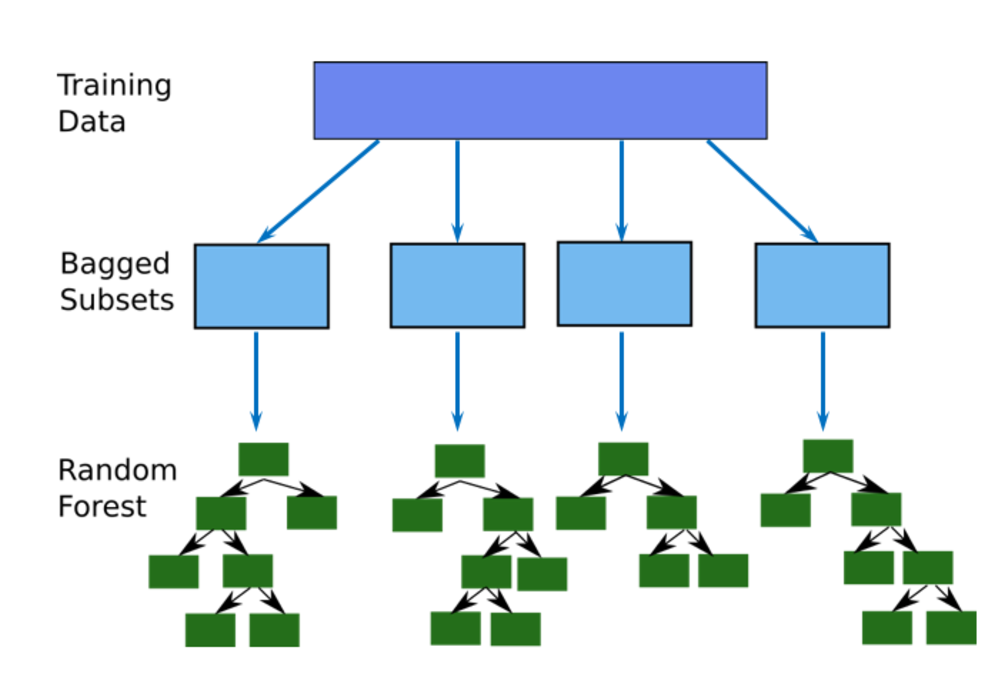
\includegraphics [width=65mm]{Images/randomforest2.eps}
%\end{center}
%\caption{Schematic of the random forest algorithm. The training data are randomly subsampled via bagging, and each bag is used to train a decision tree. All trees have an equal vote toward the final prediction.} 
%\label{fig:randomforest} 
%\end{figure}

Random forests have been applied successfully to a range of applications in materials science. They have been used to discover new Heusler compounds~\cite{Oliynyk2016} and new thermoelectric materials~\cite{Gaultois2016}. They have also been used to model material properties such as thermal conductivity in half-Heusler semiconductors ~\cite{Carrete2014} and to break down fields for dielectrics~\cite{Kim2016}. Ling et al.~\cite{Ling2017} demonstrated how random forest models with jackknife-based uncertainty estimates could be used for experimental design in materials science. The application of machine learning for experimental design is particularly compelling for AM, where there are many processing steps that affect build quality. 

Kamath utilized random forests among other machine learning techniques to predict melt pool depths based on the results of an Eagar--Tsai model for powder melting \cite{Kamath2016}. The Eagar--Tsai model uses a Gaussian laser beam incident on a metal substrate and models the temperature distribution throughout a bed of powder. Kamath was seeking to understand the most important laser parameters to use for predicting a melt pool's size and shape. Kamath started with the inputs of the Eagar--Tsai model and ordered them based on their numerical value. Then, a random forest algorithm was built that split variables based on the standard deviation of their associated output. The main idea was that variables that had a high impact would have a low standard deviation in their associated outputs. Using this method, they found that laser speed and power were the most important inputs for determining the melt pool depth and shape. After determining the most important inputs, the same regression tree was applied in order to find optimized manufacturing conditions for fully dense parts, using the same method.

Kamath's study also highlights a theme across studies of AM: the process combines separately known physics across separate domains. For example, a laser physics model will have a set of descriptors for describing the laser's behavior, while a solidification model will have a separate set of descriptors for itself. Descriptions across separately contained models do not obviously demonstrate how the descriptors interact, or which descriptors from one model are important to include in the other model. Science has long benefited from simple models, possibly empirical, which provide a small amount of physical descriptors to model specific properties. Machine learning algorithms can search through physical parameters used to model AM to find the lowest dimensional description which explains the widest swath of phenomenon. This is desirable for building computationally accessible models.

The many different computational models of AM, whether they are finite/direct element, central difference, phase field, or otherwise can all be upscaled to describe more and more physics.  Interaction potentials between forces during manufacturing can be added to models, requiring more input descriptors. Take, for example, a finite element model that describes thermal flux through a system from the interaction of a laser on a powder bed \cite{Khairallah2016}. There are many physics to consider here -- the energy transfer of the laser on the powder bed, movement of powder, phase change from powder to melt pool, thermal fluid mass transfer in the melt pool, convective, cooling, and radiative heat loss, and more. The full-physics model may have \textit{many} inputs $\mathbf{x} = (x_1,x_2,...,x_n)$ where $n$ is large.

The original, full-physics model produces a relationships $y = f(\mathbf{x})$ and may be computationally expensive, creating a bottleneck for process design and knowledge generation. A more computationally accessible model $y^*(\mathbf{x^*})$ would be desirable. In this case, the set of descriptors $\mathbf{x^*}$ consists of a subset of descriptors from $\mathbf{x}$, but is a much smaller set and requires less computational resources. 

Stated otherwise, the goal is to solve the objective function
\begin{equation}
	\text{min} ||y^*{(\mathbf{x^*})} - y(\mathbf{x})||
	\label{obj}
\end{equation}
such that $\{\mathbf{x^*} = \left(x_i...x_m\right) \in \mathbf{x} | m << n\}$

Finding the solution to Eqn, \ref{obj} can be achieved by fitting random sampling of descriptors from $\mathbf{x}$ and creating regression models on the outputs of the original model $y(\cdot)$. Presumably, the original full-physics model has been run and evaluated for accuracy. This means the researcher has a set of computationally-generated data $y$ as well as the inputs used to assess the model $\mathbf{x}$. 

Various subsets of the model inputs $\mathbf{x^*}_i$ can be chosen by randomly sampling the full list of inputs $\mathbf{x}$ repeatedly. Each subset of inputs can then be regressed upon, perhaps by using least squares regression
\begin{equation}
	\text{min} ||\mathbf{Y} - \mathbf{X^*_i} \mathbf{c_i}||
	\label{obj2}
\end{equation}
where $\mathbf{Y} = (y_1,y_2,...,y_n)$ are the outputs of the full-physics model, $\mathbf{X} = \left[ \mathbf{x^*} ,\mathbf{x^*},...,\mathbf{x^*}\right]^T$ is an $n \times m$ matrix of the subset of inputs, and $\mathbf{c}$ is a vector of weighting coefficients. This produces a randomly-generated model $y^*(\mathbf{x^*_i}) = \mathbf{X^*_i}\mathbf{c_i}$ which may or may not be able to accurately reproduce $y(\cdot)$. To find the \textbf{best} subset of inputs, one can solve 
\begin{equation}
	\underset{\mathbf{c}}{\text{min}}|| \mathbf{Y} - \mathbf{X^*_i} \mathbf{c_i}|| + \lambda||\mathbf{c_i}||
	\label{KRR}
\end{equation}
which is the objective equation for a machine learning method known as Kernel Ridge Regression (KRR). The idea behind Eqn. \label{KRR} is that it is a feasible minimization problem from a complexity perspective, i.e. it is convex. KRR is the basis of a descriptor set investigation performed by Ghiringhelli et al. to find the lowest dimensional descriptor for predicting crystal structure.They were able to identify one-dimensional, two-dimensional, and three-dimensional descriptors that were all shown to be the ``best'' combinations of descriptors out of any $n$-tuple \cite{Ghiringhelli2015}. Better physical descriptors are often found by combinatorial analysis of as many independent variables and dependent variables as possible. The `best' descriptors found experimentally are usually judged based on the amount of physics they are able to reproduce. Using descriptor analysis, as Ghiringhelli did, experimentalists can find the best descriptors as quickly as possible. Then, when trying to predict material properties in the future, researchers know which descriptors to use or combine.
\subsubsection{Surrogate Modeling}
Dimensionally reduced models are useful for engineering applications where few properties are being studied at a time, or when computational burden hinders development time considerably. Full-physics modeling is quite necessary to understand how physics at different scales interact to impact the AM process. Full physics models, however, can be expensive and time consuming to run. Phenomenon which are difficult to study experimentally, such as flow within the melt pool, are best studied through modeling approaches. If a model's computational expense is \textit{too} high then performing simulations at all relevant manufacturing conditions can be impossible. Machine learning algorithms can use the results of previously run high fidelity simulations to fill in the gaps and reduce development time.

A \textit{surrogate model} is a mathematical approximation that predicts the results of AM simulations without actually performing the computation. Surrogate models preclude the need for running computationally expensive simulations for every possible manufacturing condition. The results of previous data-intensive simulations can be used in regression models to predict the results a simulation \textit{would have} given, if it had actually been performed. Surrogate models can be as simple as linear regression between simulation inputs and results, but are often more complex. The accuracy of a surrogate model is dependent upon how many previous simulations have been run and at how many different points in the design space.

Tapia et al. built a surrogate model for laser powder bed fusion of 316L stainless steel. They were concerned with predicting the melt pool depth of single-track prints solely from the laser power, velocity, and spot size \cite{Tapia2017}. The dataset used to build the surrogate was computationally derived, based on previous simulation methods used by the same research team \cite{King2014}. In particular, they used the results from a computationally expensive but high-accuracy melt pool flow model of Khairallah et al. \cite{Khairallah2016}. They ran powder bed simulations at various laser powers, velocities, and spot sizes, and the model told them the depth of the melt pool, among other information. The datasets provided enough information for a surrogate model to be trained to predict simulation results.

To build this model, Tapia et al. used a machine learning model known as a Gaussian process model (GPM). A common model assumption in Gaussian process modeling is
\begin{equation}
	z(\mathbf{x}) = y(\mathbf{x}) + \epsilon(\mathbf{x})
	\label{model}
\end{equation}
where $y(\mathbf{x})$ is the approximation (surrogate) of the simulation process, $\epsilon(\mathbf{x})$ is a stochastic, randomly distributed noise in measurement, and $z(\mathbf{x})$ is the value given by a simulation. GPMs make the assumption that all finite joint distributions of $y(\mathbf{x})$ are distributed in a multivariate normal manner, also known as a Gaussian distribution. For AM modeling this assumption holds if the model data used for a surrogate is stochastic in nature. The primary goal in GPMs is to find model parameters for the mean process $y(\mathbf{x})$ and a covariance function $C(\mathbf{x},\mathbf{x}')$, which is a function of similar form to Eqn. \ref{guasskernel}. Fitting a Gaussian process model often begins with assuming a model function for covariance, fitting the model parameters to the observed values $z(\mathbf{x})$, then using those model parameters to predict simulation results $y(\mathbf{x})$ at other locations in the design space. 

Starting with the covariance of their inputs, Tapia used Bayesian statistics to develop a probabilistic model that predicted melt pool depth from simulation inputs. They were able to successfully predict the outcomes of both high-fidelity simulations and experimental measurements solely by analyzing trends in previously obtained results. In particular, they were able to accurately predict the melt pool depth at a value that had never been observed before, either computationally or experimentally. For future investigations, predictions by the surrogate model can be relied up on instead of running a simulation or experiment. 

Gaussian process models have benefits beyond their surrogate modeling capabilities. GPM provide robust uncertainty metrics on the predictions they make. Uncertainty in prediction is important in materials informatics because it aids in discriminating against poor prediction accuracy in machine learning. Some machine learning models do not have straightforward ways of assessing model error \cite{Bessa2017}. 

Another benefit of GPM is that it aids in inverse design and design space visualization. GPMs can explicitly identify regions of the design space which will maximize or minimize a value. In the case of Tapia et al. response surfaces were created from the GPM which visualized the depth of melt pools as a function of laser power and speed. Doing so allows engineers to identify regions of the design space which provide specific material responses, an important tool in optimization for additive.

Another approach to full scale models in AM is building high-fidelity models from an ensemble of low-fidelity models. Current integrated computational models link phenomena across spatiotemporal scales by running many single-physics models and passing the results from model to model, then comparing with experimental results. An example is the model of Martukanitz et al. that considered the thermal, mechanical, and material response of Ti-6Al-4V alloys manufactured with powder bed processes \cite{Martukanitz2014}. Martukanitz's model uses the finite element method to model the thermal and mechanical response based on classical continuum heat transfer equations. At the same time, the Calculation of Phase Diagrams (CALPHAD) method modeled the thermodynamics and mass transfer for each chemical species, while Diffusion-Controlled phase Transformations (DICTRA) is used to model phase formation. As noted by Martukanitz, this approach becomes computationally infeasible as the number of deposition layers increases.

Even a \textit{single} modeling method -- just FEA, phase field, CALPHAD, etc -- becomes computationally expensive for thousands of layers of material deposition. Based on this scaling, accurately modeling the physics of a full build seems impossible, at least without a major leap in computing power. A machine learning method known as \textit{committee voting} or \textit{ensemble modeling} may provide a workaround. These methods rely on sampling many individual models to predict the behavior of a larger class of physics.

In traditional ensemble modeling approaches, many different regression models are trained to model a relationship $y = f(\mathbf{x})$, as in regression trees. For a given input $\mathbf{x_1}$ all regression models are assessed and various outputs predicted, $f_1(\mathbf{x}), f_2(\mathbf{x}), ..., f_n(\mathbf{x})$, etc. In AM it may make more sense to use data from single-scale AM models as the base models and train a machine learning based regression model from those. These data sets for additive may be the inputs and solutions of a solidification or heat transfer model, or experimentally obtained relationships.

Ensemble modeling can be used in AM to solve multiobjective optimization problems, such as optimizing the heat transfer through a build and the grain growth simultaneously. Doing so would require training an ensemble model of simulations. The simulations to include could be thermomechanical models of heat transfer, phase field models of grain growth, finite element models of laser absorption, and so forth. The final ensemble model would take the form
\begin{equation}
	\mathbf{y}(\mathbf{x}) = \sum_{i=1}^N w_i f_i(\mathbf{x})
	\label{ensemble}
\end{equation}
where $\mathbf{y}$ is a response vector of properties to optimize, $f_i(\mathbf{x})$ is a single simulation of the process out of $N$, and $w_i$ are weights associated with each simulation. The vector $\mathbf{y}$ would contain many parameters such as temperature $T(t)$, temperature gradient $\nabla T$, solidification velocity $\nu(t)$, and many more phenomenon to monitor from simulations. 

In the AM case, where information from models may overlap, this type of approach can screen out noise from simulations or experiments to gauge a more fundamental relationship. The uncertainties associated with a model can be weighted by the experimentally observed data points. Furthermore, predictions can be made across many different physical models, resulting in a predictive method for holistic analysis of the final properties. This method does not provide a picture of how the physics in each simulation interact or disagree. However, it can be used to simultaneously optimize the results of many different simulations and point toward desirable manufacturing conditions. A review of multiobjective optimization functions can be found at \cite{Jin2008}.

Meredig et al. applied this method to the prediction of ABC ternary compounds, where A, B, and C each represent an element. \cite{Meredig2014}. The space of all combinations of A, B, and C elements is large and would require many, many simulations. Instead of running high-throughput DFT for all possibilities they used lower order simulations. Meredig ran DFT calculations for AB, AC, and BC compounds to generate a database of information. Then, regression trees were trained from the inputs of each binary alloy simulation to predict the formation energy. Finally, an ensemble model was trained
\begin{equation}
	E(\text{ABC}) = w_{\text{AB}} f(\mathbf{x}_{\text{AB}}) + w_{\text{AC}} f(\mathbf{x}_{\text{AC}}) + w_{\text{BC}} f(\mathbf{x}_{\text{BC}})
	\label{dftensemble}
\end{equation}
where $E()$ is the formation energy, $w_\text{AB}$ is the weight for a regression model of AB alloys, $f(\mathbf{x}_{\text{AB}})$ is the regression tree for all AB alloys, and so on. In the end, Meredig's model was able to predict $4,500$ new, stable ternary materials. 

Machine learning is not only limited to ex situ experimental investigations or modeling approaches. Machine learning has also made major advances in signal processing and feedback. Many of the same ideas which apply to experimental and modeling studies can also be aids for in situ analysis and feedback of the manufacturing process. 

%~%~%~%~%~%~%~%~%~%~%~%~%~%~%~%~%~%~%~%~%~%~%~%~%~%~%~%~%~%~%~%~%~%~%~%~%~
\subsection{Process Monitoring and Characterization}
Computer vision is a class of image recognition algorithms that have been developed for automated feature identification in signals. Intelligent computer vision utilizes machine learning algorithms to identify objects and features in images and time-series data. 

Monitoring of AM processes produces data equally numerous to, if not in excess of, the data produced by parametric analysis and modeling. The numerousness of time series data in AM warrants usage of quick, efficient, and robust signal processing methods for process monitoring, feedback, and control. These signal processing algorithms are closely related to machine learning. They serve as tools in their own right, and can also pre-process data for use in other machine learning applications, like clustering and regression. 

\subsubsection{In Situ Process Monitoring and Feedback}\label{sec:In Situ Process Monitoring and Feedback}
\begin{figure*}
	\includegraphics[width=0.85\linewidth]{/Users/njohnson/git/thesis/document/chapters/review/Images/Fig12_melt_pool}
	\caption{A few examples of data types, data sensors, and features to detect in a laser powder bed fusion manufacturing process. The wide range of signals to monitor then control makes feedback and control in AM especially difficult. Computer vision techniques can be applied to automatically detect features of interest across multiple data types and data sensor simultaneously.}
	\label{fig:melt_pool}
\end{figure*}

In situ monitoring, feedback, and control has been consistently ranked as one of the most-needed technologies for advancing additive manufacturing \cite{Berumen2010, Tapia2014, Mani2017}. The combination of rapid solidification and the small length scales of AM solidification can make traditional process monitoring approaches difficult. Furthermore, there are many processes/problems to monitor for during the manufacturing process, with equally as many sensor types for monitoring as shown in Figure \ref{fig:melt_pool}. Machine learning can fill in gaps that leverage correlations and relationships from previous measurements, observations, and responses.

Process monitoring involves acquisition of real-time signals that can reveal information about a wide variety of phenomenon during manufacturing. Many developments of in situ process monitoring technologies are focused on controlling a) microstructure growth or development; or b) the prevention of defect formation. 

There are in-situ experiments being performed to inform models of the additive manufacturing process. In situ experiments advance our understanding of AM, as well as advance feedback and control for AM, through several outcomes. In some cases,  in situ studies reveal what a `good' or `bad' AM process looks like. They also inform researchers of those conditions that must be met to achieve a desired outcome or prevent the formation of a defect. In situ experiments also push the development of sensor technology for AM. While sensor technology will not be covered in this review it is an important topic for the advancement of AM technology. Purtonen et al. wrote a review of common sensing methods for laser based manufacturing\cite{Purtonen2014}.

Early experiments using in situ monitoring for AM focused around either the ability to measure thermal signatures accurately or relating key features of the solidification process to important material properties. McKeown et al. has used dynamic transmission electron microscopy to measure solidification rates in powder bed AM \cite{McKeown2016}. Bertoli et al. have also characterized cooling rates using high speed imaging \cite{Bertoli2017}. Raplee et al. have used thermography to monitor the solidification and cooling rates of electron beam powder bed fusion, relating the temperature profiles to defect and microstructural characteristics \cite{Raplee2017}. Distortion of parts due to thermal cycling was investigated by Denlinger et al. by means of thermocouples in contact with the build substrate \cite{Denlinger2015}. Guo et al. used synchrotron X-ray imaging to characterize the dynamic behavior of spatter during laser-based AM \cite{Guo2018}. Leung et al. likewise used synchrotron X-ray imaging to characterize defect formation and molten pool dynamics during laser powder bed fusion \cite{Leung2018}. Based on the behavior they observed, Guo et al. were able to suggest control mechanisms for minimizing spatter during manufacture. Everton et al. provide a review of in situ monitoring for metal AM \cite{Everton2016}. All of the data being recorded in these studies can be used as \textit{features} for training machine-learning based feedback and control systems. The class of algorithms used in these cases is called computer vision.

The type of data being collected in situ is often in the form of time series or image data. In computer vision, as with traditional feedback and control, algorithms are used to identify deviations from a desired signal. The power of computer vision approaches is their ability to simultaneously monitor and identify signal changes across multiple sensor types, as well as multiple different types of deviation from a single sensor. Examples include identifying a spike in temperature or a sharp change in intensity in an image indicating a deviation from a desired processing conditions. Image processing \textit{filters} can be used to selectively modify or extract features in AM data. Image processing filters are mathematically analogous to those introduced for topology optimization (Section~\ref{sec:topology optimization}). 

A filter is implemented as a mathematical operation, a kernel, applied to a window of time series data or an area of pixels in an image. For images, as previously discussed in Section \ref{feat}, filters attempt to use local spatial information and \textit{a priori} knowledge of the expected properties of the image to improve image quality and extract features, e.g., distinctive characteristics such as edges or regions of similar intensity (domains) that represent the boundaries or spatial extents of objects, phases, etc.

AM processes span several orders-of-magnitude in both length and time scales from ejected particles moving across the field of view in milliseconds to multi-hour builds and sub-millimeter melt pools to part-scale thermal distortions. Practically, then, in situ monitoring requires compromises in data collection rates and resolutions, and data processing filters are used to reduce noise and extract features, such as melt pool width, from the as-collected data. A comprehensive review of image filters is beyond the scope of this review, so the interested reader is directed to the many works on this topic, such as Vernon et al\cite{Vernon1991}. However, three use cases are especially common and worth discussion here: reduction of high-frequency noise, also known as salt-and-pepper noise; additive noise reduction; and edge detection.

High frequency noise is characterized by sudden changes in intensity relative to the surrounding field. Although there are a number of possible causes, this may be caused by pixel-level variability or insufficiency in the detector, e.g. ``dead pixels'' or excessive gain. Median and conservative filters are commonly used when the fraction of noise pixels is large (1\%--10\%) and small ($<$ 1\%), respectively.

Additive noise, unlike high frequency noise, is a result of insufficient counting statistics, which may result from insufficient exposure time, or detector efficiency. A gaussian filter adjusts the intensity of each pixel according to the weighted intensities of neighboring pixels. Unlike median and conservative filters, a gaussian filter will soften edges, making adjacent domains less distinct.

Filters also have applications beyond noise reduction, primarily in object and feature detection. Detecting phenomena of interest during manufacturing is the first step to feedback and control mechanisms. Edge detection captures local changes in intensity to identify transitions between adjacent domains. Laplacian or Laplacian of Gaussian (LoG) filters themselves are sensitive to noisy images, identifying spurious edge artifacts, but are used as part of larger algorithms, such as Canny edge detection~\cite{Canny1986}. Canny edge detection include noise reduction to mitigate artifacts of LoG filters, and can be used to monitor melt pool shape and identify other features, such as unmelted powder particles attached to the build surface. Canny edge detection, along with other feature extraction algorithms, can be used to extract the features that characterize the build and can be used as part of a larger machine learning workflow to classify build quality. For example, these features can be used in learning algorithms to correlate characteristic features, such as melt pool width and hatch spacing, with particular behaviors, such as the formation of lack of fusion defects, in the manufacturing process. In this case, identification of a feature, or set of features, may be sufficient to indicate a particular process outcome.

Template matching is a computer vision method that can be used for automatic identification of common patterns. It involves the comparison of an unclassified input to a database of pre-identified patterns. For AM, template features include abnormal melt pool morphologies \cite{Kanko2016}, inclusion of unmelted powder particles \cite{Yang2017}, and denudation near the melt zone \cite{Matthews2016}. The scale-invariant feature transform (SIFT) \cite{Lowe2004} and a variant, ``Speeded-Up Robust Features'' (SURF) \cite{Bay2008} are both feature identification algorithms that can be used for template matching. Another template matching algorithm is the \textit{bag of visual words} or dictionary method~\cite{DeCost2015}. A collection (dictionary) of typical features from the AM process can be built based on features obtained from filters. The features measured in situ are compared with dictionary entries. If an in situ feature matches a defect-indicative feature from the dictionary, then it is likely a defect has formed during manufacturing.

\begin{figure}
	\includegraphics[width=0.48\textwidth]{/Users/njohnson/git/thesis/document/chapters/review/Images/Fig13_ActivationFunctions}
	\caption{Common activation functions in artificial neural networks (NNs) that introduce nonlinearity into the NN. The sigmoid is the archetype activation function because the closed form solution for the derivative of the sigmoid, which is used during model fitting, is an excellent pedagogical tool; however, the rectified linear unit (ReLU) is, at present, the most common activation function in the hidden layers of NN. Uses for the other activation functions are provided in the text.}
	\label{fig:activation functions}
\end{figure}

Neural networks (NNs) are particularly well-suited to handle features extracted from images, or simply the images themselves. There are many references that describe neural networks in detail, such as the work of Hastie et al\cite{Hastie2009}, and an increasing number that address the specific challenges associated with neural networks in materials science~\cite{Bhadeshia2009}. There are several properties of NNs that are worth repeating here, however. Each layer in a NN is connected to the next layer through an affine (linear) transformation. This step stretches, scales, and skews the input vector.
\begin{equation}
	{\bold z}^{(i+1)} = \boldsymbol \theta_i^T {\bold x}^{(i)}
\end{equation}
where ${\bold z}^{(i+1)}$ is the input into the $(i+1)$ layer and ${\bold x}^{(i)}$ is the output from the previous, $i^\textrm{th}$ layer. Then, an activation function, such as those summarized in Figure~\ref{fig:activation functions}, introduces a non-linearity that warps/distorts the vector input to that layer.

\begin{equation}
	{\bold x}^{(i+1)} = f \left( {\bold z}^{(i+1)} \right)
\end{equation}

The model parameters $\mathbf{\theta}_i^T$ are regression weights that associate outputs from each layer $\mathbf{x}^{(i)}$ to subsequent layers $\mathbf{z}^{(i + 1)}$. By increasing the depth of the NN, that is, adding additional layers, and the width (number of nodes) of those layers, a NN can be used to approximate any function, making them powerful regression and classification tools~\cite{Hornik1989}. However, the general sparsity of materials data coupled to the complexity of process--structure--process relationship requires an understanding of the tradeoffs and requirements of using NNs in materials science, and in AM more specifically. Beyond the basics of model architecture, overfitting and the bias--variance tradeoff that is part of any machine learning model, a basic understanding of the role of activation functions can help to develop an intuition for the use of NN in materials and manufacturing.

An early use of NNs was in classification. The perceptron, logistic sigmoid (or simply, sigmoid), and hyperbolic tangent are all activation functions that choose between two options (0 or 1, or in the case of $\tanh$, -1 or 1). While a binary option may seem overly limiting, even multinomial classification can be broken down into a sequence of such binary classificiations: \textit{A} or not \textit{A}; and if not \textit{A}, then \textit{B} or not \textit{B}; and if not \textit{B}, \textit{C} or not \textit{C}; etc. However, such a serial solution will require more layers and, with more layers, longer training on larger datasets to fit all model parameters.

Visual examples of these activation functions can be seen in Figure \ref{fig:activation functions}. While each behaves differently, particularly across the negative domain ($x < 0$), the simplicity and robustness of the ReLU have made it the most commonly used activation function for hidden layers in regression neural networks.

In the case of a multinomial classification problem, a more simple network may be possible by using one-hot encoding. A one-hot encoding vector is defined for $N$ exclusive options: one element in the $N$-element vector is 1, all other values are 0. Rather than using multiple layers to construct the binomial ladder required to simulate a multinomial decision, the softmax activation function selects one-from-many in a single layer. Since each value in the input vector appears in the softmax exponent, even small differences in the magnitude of $z$ result in large differences in the output of this activation function; therefore one option, represented by one node or neuron in the layer, is approximately 1 and all others are nearly 0. Simplification of the network architecture by choosing activation functions that more closely resemble the nature of the problem emphasizes the importance of domain-specific knowledge in developing appropriate NN architectures.

Combining the concepts of neural networks and image processing filters, convolutional neural networks (CNNs) not only learn how to correlate features to results, they are designed to also identify the filters that extract those features. These networks require large numbers of parameters, in the tens to hundreds of millions, that introduces an insurmountable training burden due to the sparsity of materials data. However, CNNs trained on natural images have demonstrated a remarkable similarity in their initial layers~\cite{Yosinski2014}. These first few layers identify basic shapes, edges, and colors that are common to many image types; a phenomenon that many groups have exploited to overcome the limitation of data sparsity through transfer learning~\cite{Ling2017a}, including specific work in the field of additive manufacturing. Yuan et al \cite{Yuan2018} were able to successfully monitor melt track width, standard deviation, and continuity of tracks in situ during laser powder bed manufacturing. Scime and Beuth trained a convolutional neural network to identify six different types of defect that are typical of laser powder bed fusion, with reasonable prediction accuracy \cite{Scime2018}. Li et al. used a type of neural network method called \textit{deep learning} to classify AM parts using microstructural images \cite{Li2020}. Kwon et al. classified melt pool morphologies using a neural network \cite{Kwon2018}. These studies represent only a few possible uses of CNN for in situ process monitoring of AM.

Scime and Beuth modified a well-known convolutional neural network architecture -- known as AlexNet \cite{Krizhevsky2012} -- to perform classification of powder spreading errors that occur in laser powder bed fusion \cite{Scime2019}. The study presented by Scime and Beuth go in-depth on the architecture of their CNN and directly explain how the training of filters applies in the context of AM images. 

\subsubsection{Featurization of Qualitative Image Data}
The use of images in studying additive manufacturing is widespread, common throughout all aspects of the manufacturing process, and provides key information about material properties and processing. As with all aspects of AM, the sheer size of image data to be analyzed is profound due to the large design space of AM. The types of information taken from images includes grain characteristics, like size, orientation, and phase, and defect characteristics, like pore size or crack length. When characterizing all of these features for all possible processing conditions and alloys the size of the problem grows quickly.

Computer vision algorithms have been tested for automation of materials science image classification and analysis. Using these algorithms can speed up the experimental characterization process of AM. Furthermore, computer vision techniques can quantify information which may have otherwise only been used qualitatively or measured by approximation. 

It is worthwhile to mention up front that these algorithms have been \textit{tested} on microstructure and, in some cases, additive-specific images. There are few algorithms that can process AM microstructure data `out-of-the-box.' Rather, these algorithms will need to be tailored in order to quantify AM images specifically. However, the algorithms discussed here have been proven on non-AM microstructure datasets, thus they should be extensible to AM datasets. The computer vision approaches which work for microstructure data are often the same approaches discussed in the previous section for in situ monitoring. 

One AM-related application of image characterization is measuring particle size distributions in AM powder feedstock. DeCost and Holm used SIFT with a dictionary classifier, as in template matching, to measure the particle size distribution for a dataset of synthetic powder particles \cite{DeCost2017a}. Particle size distribution plays in several steps across the additive process including energy absorption and part metrology \cite{Zhou2009, Boley2015, Boley2016}. DeCost created datasets with six different particle size distributions. Image features were identified and classified using $k$-means clustering on the features found by SIFT. Then, a classification algorithm known as a support vector machine (SVM) was trained to classify image features into particle sizes. DeCost was able to achieve $89$\% overall classification accuracy in measuring particle size distribution this way. DeCost et al. later improved upon this powder classification method and were able to achieve higher classification accuracies for real powder images \cite{DeCost2017}.

Strides have been made in automatically identifying and quantifying information from metallographs \cite{DeCost2015, DeCost2017b, Ling2017a, Bulgarevich2018}. A good portion of quality control in materials science as a whole, not just AM, involves classifying materials based on metallographs or micrographs of microstructure. Work is being done across materials science to apply machine learning based computer vision to classifying and quantifying information in these microstructural images. Doing so will speed up the process of materials characterization and qualification, while also providing methods of quantifying information which otherwise would have stayed in a qualitative form. Examples include classification of grain stuctures, measurements of grain size, pore size calculations, and more.

An additive-specific image segmentation algorithm was used by Miyazaki et al. \cite{Miyazaki2019}. Five image filters were convolved with microstructure images of selective laser melted Ti-6Al-4V. The features identified by these filters were used in a random forest algorithm to segment the image into regions of $\alpha$ phase grains and $\beta$ phase grains. The algorithm was able to automatically calculate area fraction of primary and secondary $\alpha$ phases that form during cooling. It was also able to calculate the nearest-neighbor distance between grains. Nearest neighbor distance of grains is indicative of grain characteristics like size, morphology, and distribution. 

Chowdhury et al. took a more expansive approach to performing feature identification in microstructures. In particular, they were looking to classify microstructures as either dendritic or non dendritic. Chowdhury employed 8 different feature identification methods for a dataset of images. Classification was performed using an ensemble of ML techniques including support vector machines (SVM), Na\"ive Bayes, nearest neighbor, and a committee of the three previous classification methods \cite{Chowdhury2016}. Chowdhury's wide approach to image classification achieved classification accuracies above 90\%. 

It would be overly burdensome to lay out every \textit{possible} application of computer vision in additive manufacturing. Efforts are underway across materials science to implement computer vision for the automation of materials classification. Rather, the authors would like to refer the reader to reviews on the subject of computer vision for materials science, as well as open libraries listed in Table \ref{data_tools}. The hope is that readers will discover the many possible uses of computer vision and begin applying methods to their own AM problems. 



 


